% -----------------------------------------------
% Template for ISMIR Papers
% 2018 version, based on previous ISMIR templates

% Requirements :
% * 6+n page length maximum
% * 4MB maximum file size
% * Copyright note must appear in the bottom left corner of first page
% * Clearer statement about citing own work in anonymized submission
% (see conference website for additional details)
% -----------------------------------------------

\documentclass{article}
\usepackage{ismir,amsmath,cite,url}
\usepackage{graphicx}
\usepackage{color}


% Title.
% ------
\title{TimeSide, a scalable audio processing framework and REST API written in Python}

% Note: Please do NOT use \thanks or a \footnote in any of the author markup

% Single address
% To use with only one author or several with the same address
% ---------------
%\oneauthor
% {Names should be omitted for double-blind reviewing}
% {Affiliations should be omitted for double-blind reviewing}

% Two addresses
% --------------
%\twoauthors
%  {First author} {School \\ Department}
%  {Second author} {Company \\ Address}

%% To make customize author list in Creative Common license, uncomment and customize the next line
%  \def\authorname{First Author, Second Author}


% Three addresses
% --------------
% \oneauthor
%   {Guillaume Pellerin} {IRCAM, France \\ {\tt guillaume.pellerin@ircam.fr}}

\threeauthors
  {Guillaume Pellerin} {IRCAM Lab, CNRS, \\ Sorbonne Universit\'es, France \\ {\tt \small guillaume.pellerin@ircam.fr}}
  {Josephine Simonnot} {CREM / LESC, CNRS, \\ Universit\'e Paris Nanterre, France \\ {\tt \small josephine.simonnot@cnrs.fr}}
  {Thomas Fillon} {RTSYS, France \\ {\tt \small thomas.fillon@gmail.com}}
  
%% To make customize author list in Creative Common license, uncomment and customize the next line
%  \def\authorname{First Author, Second Author, Third Author}

% Four or more addresses
% OR alternative format for large number of co-authors
% ------------
%\multauthor
%{First author$^1$ \hspace{1cm} Second author$^1$ \hspace{1cm} Third author$^2$} { \bfseries{Fourth author$^3$ \hspace{1cm} Fifth author$^2$ \hspace{1cm} Sixth author$^1$}\\
%  $^1$ Department of Computer Science, University , Country\\
%$^2$ International Laboratories, City, Country\\
%$^3$  Company, Address\\
%{\tt\small CorrespondenceAuthor@ismir.edu, PossibleOtherAuthor@ismir.edu}
%}
%\def\authorname{First author, Second author, Third author, Fourth author, Fifth author, Sixth author}


\sloppy % please retain sloppy command for improved formatting

\begin{document}

%
\maketitle
%
\begin{abstract}
TimeSide is an open source audio processing framework written in Python enabling low and high level audio analysis, imaging, transcoding, streaming and labeling. Its high-level API is designed to enable complex processing on very large datasets of any audio or video assets with a plug-in architecture, an secure extensible backend and an dynamic web frontend. It embeds many state-of-the-art processing libraries, a RESTFul API and a Docker composition in order to be used as a scalable web service installable in a few minutes. The potential use cases are : scaled audio computing (feature extraction, filtering, machine learning, etc), web audio visualization, fast audio process prototyping, realtime and on-demand transcoding and streaming over the web, automatic segmentation and labeling synchronized with audio events. In this paper, some experimental as well as production examples will be presented on the basis of collaborative web platforms where computational musicology methods are targeted. It will be shown in particular how the framework resolves some usual problems dealing with a large number of dependencies, versioned data and human inputs in the field of reproducible research and production.
\end{abstract}


\section{Introduction}

\subsection{Context and motivation}

As the number of online audio applications and datasets increase, it becomes crucial for researchers to be able to prototype and test their own algorithms as fast as possible on various platforms. On the other side, content providers and producers need to enhance user experiences on their platform with more metadata based on cultural history but also acoustical and high level semantical analyses from the audio signals. Growing those metadata synchronously with the music published on the internet implies that the analysis and storage systems can easily be scaled and deployed. Because in the open source context such systems can have a hundreds of dependencies, it therefore becomes crucial to have a framework architecture that allows such a dynamic and flexible behavior where each bundled dependency can be easily managed and installed in a independant but also be pinned and then freezed sometimes.

\subsection{Streaming and on demand Processing}

A Web oriented analysis framework has also to deal with an environment of data that changes a lot and fast. That is, if the users can upload some large datasets, the system should respond as soon as possible as the user browses its own data, not waiting for all analyses to be acommplished. This user oriented approach allows to design to interfaces where informations will be obtained on demand, i.e. through streaming protocols that give access to data on the fly. 

\subsection{Fast Prototyping and Versioned Data}

To be evolutive, the framework should also provide an simple API for prototyping algorithms without having to re-write decoders or compile any usual processor, that is, using an interpreted, object oriented language that allows inheritance and offers the state-of-the-art of MIR and machine learning tools available. All processors should be versioned so that each software resource and resulting data is managed through time.

\subsection{Sharing, Deploying and Scaling}

Another important aspect of a system allowing computation on large datasets is the ability to be easily deployed and scaled on servers in a reproducible way dealing with a large number of software dependendies. It means that every version or configuration of a piece of software needs to be setup automatically when building and deploying the images. The system hosting the service needs also to be scalable so that the persistent data can survive through the growing of repositories.

We propose and publish a new framework based on the state-of-the-art data analysis and packaging applications which enable this flexibily from the prototype to the production. The main goals are:

\begin{itemize}
 \item Do asynchronous and fast audio processing with Python (because we love it)
 \item Decode audio frames from \textit{any} audio or video media format into numpy arrays
 \item Analyze audio content with some state-of-the-art audio feature extraction libraries like Aubio, Yaafe, VAMP, Essentia as well as some pure python processors
 \item Visualize sounds with various fancy waveforms, spectrograms and other cool graphers
 \item Transcode audio data in various media formats and stream them through web apps
 \item Serialize feature analysis data through various portable formats
 \item Playback and interact on demand through a smart high-level HTML5 extensible player
 \item Index, tag and annotate audio archives with semantic metadata
 \item Deploy and scale your own audio processing engine through any infrastructure
\end{itemize}


\section{Implementation}

TimeSide is a framework developed in Python which embeds various Python, C and C++ librairies with such bindings that allows many types of data processing and management, but also a real web server which offers a REST API that can be requested by distant clients and web services. The framework is currently published\footnote{\tiny{\url{https://github.com/Parisson/TimeSide}}} under the terms of the AGPL v3 licence. 

\subsection{The TimeSide bundle}

Because there are a lot of tools available in the Python ecosystem dedicated to MIR, machine learning and data analysis, we decided to embeds all main ones. TimeSide currently bundles: Aubio\cite{aubio}\cite{BrossierPhD}, Yaafe\cite{yaafe_ISMIR2010}, Essentia\cite{essentia}, VAMP\cite{vamp-plugins}, librosa\cite{librosa}, GStreamer, TensorFlow, Torch, PyTorch, scikit-learn, Jupyter, Pandas and Pytables. They are used to develop native TimeSide plugins though its simple processing API.

\subsection{The TimeSide Plugin API}

The plugin API is based on a input/output framing methodology to ensure data streaming between each processors. Each Processor implements the following \verb|IProcessor| API class: 

\begin{lstlisting}
class IProcessor(Interface):

    """Common processor interface"""

    @staticmethod
    def id():
        """Short alphanumeric, lower-case string which uniquely identify this processor, suitable for use as an HTTP/GET argument value, in filenames, etc..."""

    def setup(self, channels=None, samplerate=None, blocksize=None, totalframes=None):
        """Allocate internal resources and reset state, so that this processor is ready for a new run.

        The channels, samplerate and/or blocksize and/or totalframes arguments may be required by processors which accept input. An error will occur if any of these arguments is passed to an output-only processor such as a decoder.
        """

    def channels(self):
        """Number of channels in the data returned by process(). May be different from the number of channels passed to setup()"""

    def samplerate(self):
        """Samplerate of the data returned by process(). May be different from the samplerate passed to setup()"""

    def blocksize():
        """The total number of frames that this processor can output for each step in the pipeline, or None if the number is unknown."""

    def totalframes():
        """The total number of frames that this processor will output, or None if the number is unknown."""

    def process(self, frames=None, eod=False):
        """Process input frames and return a (output_frames, eod) tuple. Both input and output frames are 2D numpy arrays, where columns are channels, and containing an undetermined number of frames. eod=True means that the end-of-data has been reached.

        Output-only processors (such as decoders) will raise an exception if the frames argument is not None. All processors (even encoders) return data, even if that means returning the input unchanged.
        """

    def post_process(self):
        '''
        Post-Process data after processign the input frames with process(). Processors such as analyzers will produce Results during the Post-Process
        '''

    def release(self):
        """Release resources owned by this processor. The processor cannot be used anymore after calling this method."""

    def mediainfo(self):
        """
        Information about the media object (uri, start, duration)
        """

    @staticmethod
    def uuid():
        """Return the UUID of the processor"""

    @staticmethod
    def description():
        """Return a string describing what this processor is meant for. The description should provide enough information to help the end user.
        """
    
    @staticmethod
    def version():
        """Return a string correponding to the version of the processor.
        """
    
\end{lstlisting}

To enable the real \textit{plugin} capability, a namespace is provided so that any python modules that installs a timeside/plugins directory automatically provides the processors listed in that directory. This allows to develop TimeSide plugins in independent repositories and modules, even compiled ones.


\subsection{Processors}

The framework already provides some native processors based on the plugin API.

\subsubsection{decoders}

\verb|array_decoder| (decoder taking numpy array as input), \verb|file_decoder| (file decoder based on Gstreamer), \verb|live_decoder| (live source decoder)

The usage of the Gstreamer framework through its python bindings allows the decoder to process any video or audio format from a URL. This is really useful for analyse distant resources on the Web, even YouTube video without downloading them. The decoded data are stream to the following processor as numpy arrays.

\subsubsection{encoders} 

\verb|live_encoder| (Gstreamer-based Audio Sink), \verb|flac_encoder| (FLAC encoder based on Gstreamer), \verb|vorbis_encoder| (OGG Vorbis encoder based on Gstreamer) and then \verb|mp3_encoder|, \verb|vorbis_encoder|, \verb|opus_encoder|,  \verb|wav_encoder| and \verb|webm_encoder|. Note that we could define any encoder available in the Gstreamer framework. 

\subsubsection{analyzers}

In the core module:

\verb|mean_dc_shift| (Mean DC shift analyzer), \verb|level| (Audio level analyzer), \verb|aubio_melenergy| (Aubio Mel Energy analyzer), \verb|aubio_mfcc| (Aubio MFCC analyzer), \verb|aubio_pitch| (Aubio Pitch estimation analyzer), \verb|aubio_specdesc| (Aubio Spectral Descriptors collection analyzer), \verb|aubio_temporal| (Aubio Temporal analyzer), \verb|yaafe| (Yaafe feature extraction library interface analyzer), \verb|spectrogram_analyzer| (Spectrogram image builder with an extensible buffer based on tables), \verb|onset_detection_function| (Onset Detection Function analyzer), \verb|spectrogram_analyzer_buffer| (Spectrogram image builder with an extensible buffer based on tables, \verb|waveform_analyzer| (Waveform analyzer).\newline

High level detectors available in the TimeSide-DIADEMS module\footnote{\tiny{\url{https://github.com/ANR-DIADEMS/timeside-diadems}}} :

\verb|labri_speech_music_noise| (Labri Singing voice detection), \verb|labri_speech_music_noise| (Labri Speech/Music/Noise detection), \verb|limsi_sad| (Limsi Speech Activity Detection Systems), \verb|limsi_diarization| (Limsi dirization detection), \verb|irit_singing_turns| (IRIT Singing turns), \verb|irit_harmo_tracking| (IRIT Harmonic tracking), \verb|irit_harmo_cluster| (IRIT harmonic clustering), \verb|irit_monopoly| (IRIT Mono / polyphony detector), \verb|irit_startseg| (Segmentation of recording sessions into 'start' and 'session' segments), \verb|irit_singing| (IRIT sing detection), \verb|irit_speech_4hz| (Speech Segmentor based on the 4Hz energy modulation analysis), \verb|irit_speech_entropy| (Speech Segmentor based on Entropy analysis), \verb|irit_tempogram| (IRIT Tempogram).


\subsubsection{Graphers}

TimeSide can build sized images based on analyzers results. If a given grapher depending on an analyzer is requested, the analyzer will be automatically instanciated and seamlessly added to the pipeline. The figure \ref{fig:speech} shows an example of grapher output based on the IRIT Spech Detection algorithm on a audio item\footnote{\tiny{\url{http://diadems.telemeta.org/archives/items/CNRSMH_I_2013_201_001_01}}} from the CREM's archives and the figure \ref{fig:monopoly} an example of Mono/Polyphony detection on the item \footnote{\tiny{\url{http://diadems.telemeta.org/archives/items/CNRSMH_I_2000_008_001_04/}}}.

\begin{figure}
 \centerline{\framebox{
 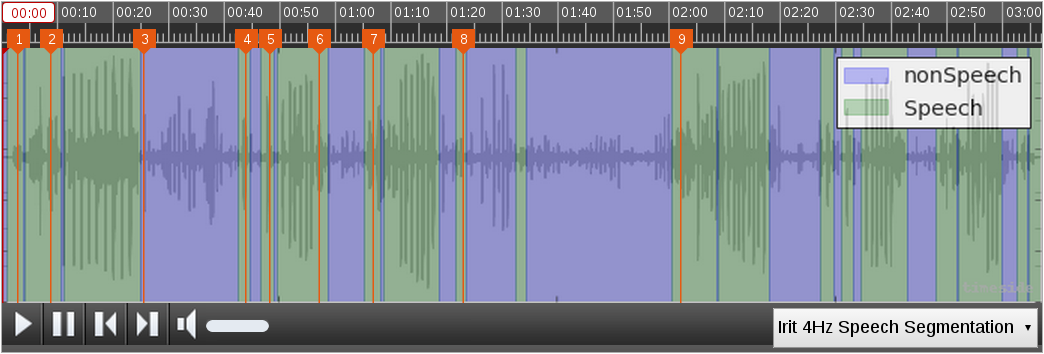
\includegraphics[width=\columnwidth]{figs/IRIT_Speech4Hz.png}}}
%  
\includegraphics[width=0.25\linewidth]{figs/CNRSMH_I_2013_201_001_01-QR.png}
 \caption{Example of a TimeSide grapher output based on the IRIT speech activity detection. Manual markers are produced before analysis.}
 \label{fig:speech}
\end{figure}

\begin{figure}
 \centerline{\framebox{
 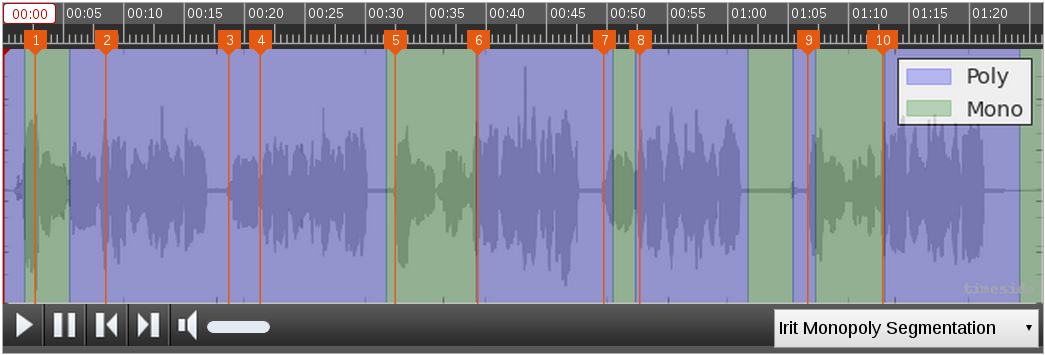
\includegraphics[width=\columnwidth]{figs/SOLO_DUOdetection.png}}}
%  
\includegraphics[width=0.25\linewidth]{figs/CNRSMH_I_2013_201_001_01-QR.png}
 \caption{Example of a TimeSide grapher output based on the IRIT Mono/Polyphony detection. Manual markers are produced before analysis.}
 \label{fig:monopoly}
\end{figure}


\subsubsection{Example analyzer}

As an example of processor definition, here is the definition of a the \verb|mean_dc_shift| analyzer:

\begin{lstlisting}
from timeside.core import implements, interfacedoc
from timeside.core.analyzer import Analyzer
from timeside.core.api import IValueAnalyzer
import numpy

class MeanDCShift(Analyzer):

    """Mean DC shift analyzer"""
    implements(IValueAnalyzer)

    @interfacedoc
    def setup(self, channels=None, samplerate=None,
              blocksize=None, totalframes=None):
        super(MeanDCShift, self).setup(
            channels, samplerate, blocksize, totalframes)
        self.values = numpy.array([0])

    @staticmethod
    @interfacedoc
    def id():
        return "mean_dc_shift"

    @staticmethod
    @interfacedoc
    def name():
        return "Mean DC shift Analyzer"

    @staticmethod
    @interfacedoc
    def unit():
        return "%"

    def process(self, frames, eod=False):
        if frames.size:
            self.values = numpy.append(self.values, numpy.mean(frames))
        return frames, eod

    def post_process(self):
        dc_result = self.new_result(data_mode='value', time_mode='global')
        dc_result.data_object.value = numpy.round(
            numpy.mean(100 * self.values), 3)
        self.add_result(dc_result)
\end{lstlisting}

A packaged dummy analyzer\footnote{\tiny\url{https://github.com/Parisson/TimeSide-Dummy}} is privided as a boilerplate to develop new plugins.

\subsubsection{Pipelining}

To enable multiple processor instanciation and processing in one decoding pass, we provide a pipe style grammar. Here is an example of some processor instanciation and then the pipe building and running:

\begin{lstlisting}
from timeside.core import get_processor

decoder  =  get_processor('file_decoder')('sweep.wav')
grapher  =  get_processor('waveform_simple')()
analyzer =  get_processor('level')()
encoder  =  get_processor('vorbis_encoder')('sweep.ogg')

(decoder | grapher | analyzer | encoder).run()

grapher.render(output='waveform.png')
\end{lstlisting}

\begin{figure}
 \centerline{\framebox{
 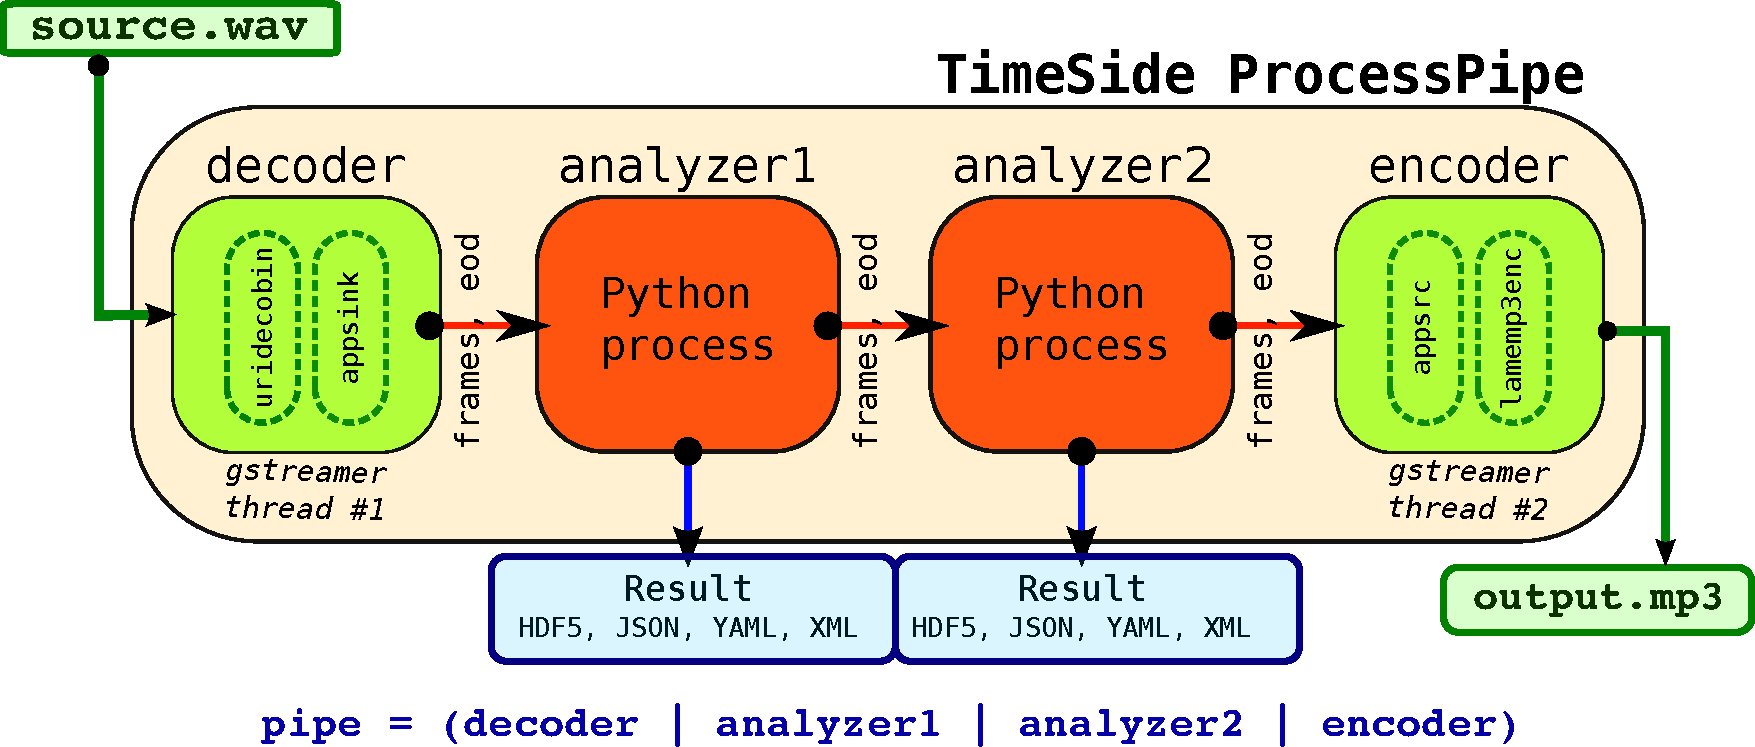
\includegraphics[width=\columnwidth]{figs/TimeSide_pipe.pdf}}}
 \caption{TimeSide pipelining example with a decoder, two analyzers and an MP3 encoder in series.}
 \label{fig:timeside_pipe}
\end{figure}

TimeSide now only allows parallel pipelining grammar but serial constructions are accessible through the Yaafe module and somehow between the parent TimeSide classes.

More examples and tutorials are proposed in the official documentation\footnote{\tiny\url{https://github.com/Parisson/TimeSide#documentation}}.

\subsection{The TimeSide Web RESTFul API}

\subsubsection{Architecture}

The TimeSide server architecture is based on the Django framework and the Django REST framework.

\subsubsection{Models and Serializers}

Models are defined as usual Django models and are all stored with a UUID. Here is a list of the main ones:

\begin{itemize}
 \item \textit{Item}: a resource with a source file or URL
 \item \textit{Selection}: a list of Items
 \item \textit{Processor}: a versioned TimeSide Processor
 \item \textit{Preset}: a Processor with some parameters in the JSON format
 \item \textit{Experience}: a list of Presets
 \item \textit{Task}: a list of Selection linked to an Experience to run
\end{itemize}

This modelization allows to define some specific precessing \textit{Experiences} that can be re-processed on any new \textit{Selection} which is espacially convenient for analysis on growing datasets. All model instances and related data are accesible through a REST API with authentication. This ensures that a client can consume TimeSide as a dedicated and autonomous web service.

The figure \ref{fig:TS2_API_UI} shows an example of the UI in front of the REST API with various URIs for each resulting resource. But of course, this API can be accessed through any distant client service or third party library (curl, coreapi, etc.).

\subsubsection{Results and Formats}

All processing results are accesible in a \verb|AnalyzerResult| python object containing a structured and documented data dictionary which can be serialized, stored and restored in HDF5, JSON, YAML or XML formats. The file contains all the preset parameters and data structure so that, if a process is requested for the same media file, same processors type and same version, the data will be automatically retrieve from the databasen and eventualluy re-processed in another child processor or serializer. The TimeSide server also embeds a full relational database to store any lighter data that has be be linked to models.

\subsection{The TimeSide Composition}

To allow reproducible building and installation and immutable application instanciation, TimeSide is bundled in a complete Docker composition which also contains all the micro-services needed to run the core engine (Python and librairies), the server (Django and modules), the worker (idem), the Notebook (Jupyter), the database (MySQL or Postgresql), the message broker (Redis) and the web server (Nginx). This packaging ensures that the application can be run on any platform and controlled with various continous integration services. Hence, starting the whole application is as simple as :\newline

\verb|$ docker-compose up|\newline


\begin{figure}
 \centerline{\framebox{
 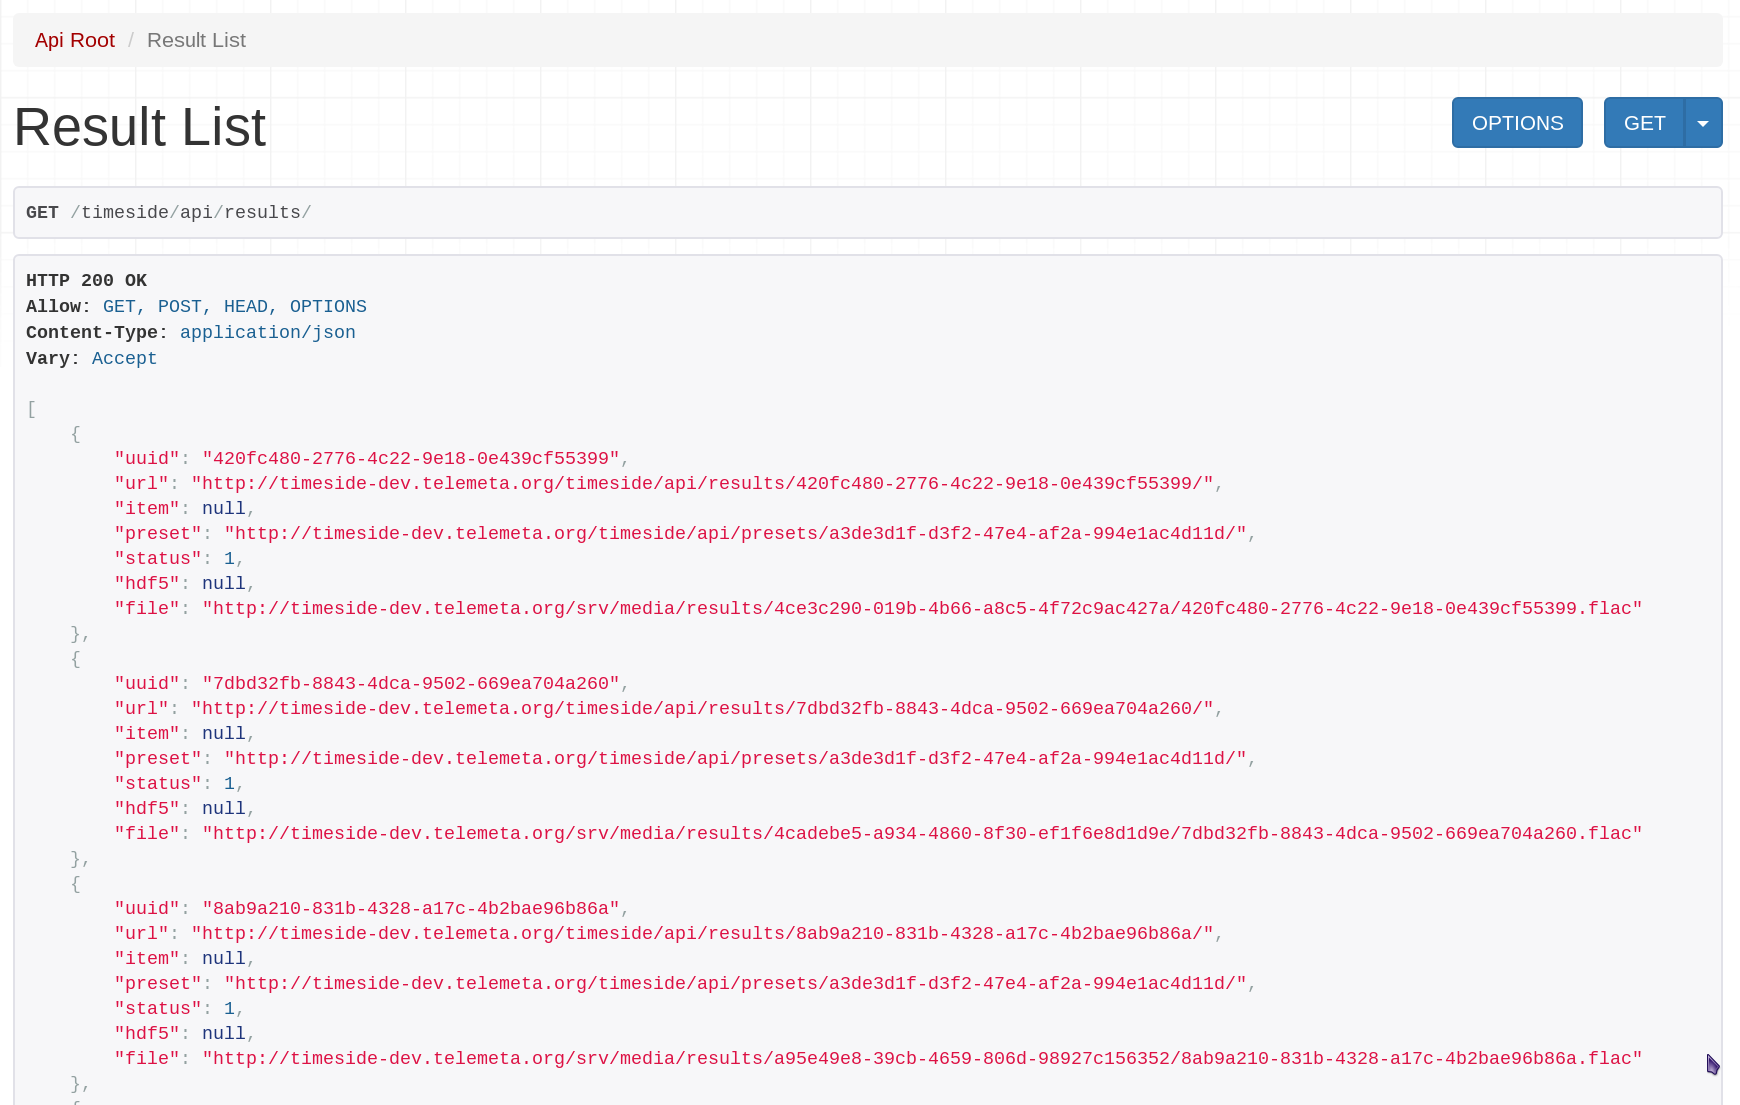
\includegraphics[width=0.93\linewidth]{figs/TS2_API.png}}}
 \caption{TimeSide REST API UI.}
 \label{fig:TS2_API_UI}
\end{figure}

\subsection{Scaling}

In applications where more than one worker is needed for asynchronous and parallel computation, the worker can be scaled through a bunch of independant threads which will be feeded by the broker. This can be applied on local CPUs as well as a Docker Swarm cluster. For example, to scale the worker on 128 threads:\newline

\verb|$ docker-compose scale worker=128|


\section{Usecases}

\subsection{Computational Musicology}

This project has been initiated during the early development stage of Telemeta\cite{telemeta} which is the first open source a collaborative multimedia platform dedicated to musicology. It has been started in 2007 from the need to publish the huge musical archives of the CNRS - Musee de l'Homme\cite{telemetaCREM}. The main idea was to associate the cultural, historical, geographical and technical metadata with the digitized audio and video files on a collaborative platform so that musicology researchers can aggregate some data, listen, annotate and, in parallel, the computer scientists can develop, test and deploy some special algorithms on original datasets edited and annotate by some experts. TimeSide has then been at the beginning of what is called now Computional Ethnomusicology\cite{Tzanetakis_2007_JIMS}\cite{Simmonot_IASA_2011}\cite{Julien_IASA_2011}\cite{Simonnot_ICTM_2014}\cite{Pellerin_AES_2014} and more recently MIRchirving. 


\begin{figure}
 \centerline{\framebox{
 \includegraphics[width=0.93\linewidth]{figs/telemeta_screenshot_en_2.png}}}
 \caption{TimeSide player integration in the Telemeta interface.}
 \label{fig:telemeta}
\end{figure}


\subsection{Large Scale Noisy Audio Analysis through the Web}

Some of the implemented plugins has been developped in the context of the DIADEMS project\footnote{\tiny\url{https://www.irit.fr/recherches/SAMOVA/DIADEMS/fr/welcome/}},: \textit{Description, Indexation, Access to Sound and Ethnomusicological Documents} in order to provide to TimeSide existing technologies, such as speech and music detections, speakers segmentation. These tools aim at extracting homogeneous segments of interest for the users. These systems have been regularly tested during numerous (inter)national evaluation compaigns, with increasingly difficult contexts, However none of these compaigns contains such diversity as there exist in the audion archives studied in this project. This heterogeneity is linked to the recording conditions, to the kind of the documents, as well as their geographical origin. The challenge for all these state-of-the-art systems is therefore to adapt them to the users needs. It has been also forseen to propose new tools for exploring the contents of the homogeneous segments. The research on the singing/speaking voice oppositin, the singing voice, the singing turns and the musical similarity are not achieved yet. A real research study on defining relevant features and how to take them into account has still to be carried out. To be able to interact with musicologists and ethnomusicologists is a major advantage in this context. During this project, a revised version of the TimeSide player has been re-designed has shown in the sketched figure \ref{fig:ts_player_v2} and is now in developement. The goal is to obtain a player capable for playing an audio files of any length (i.e. hours) and offering a better interface to edit, process and annotate archives collaboratively.

\begin{figure}
 \centerline{\framebox{
 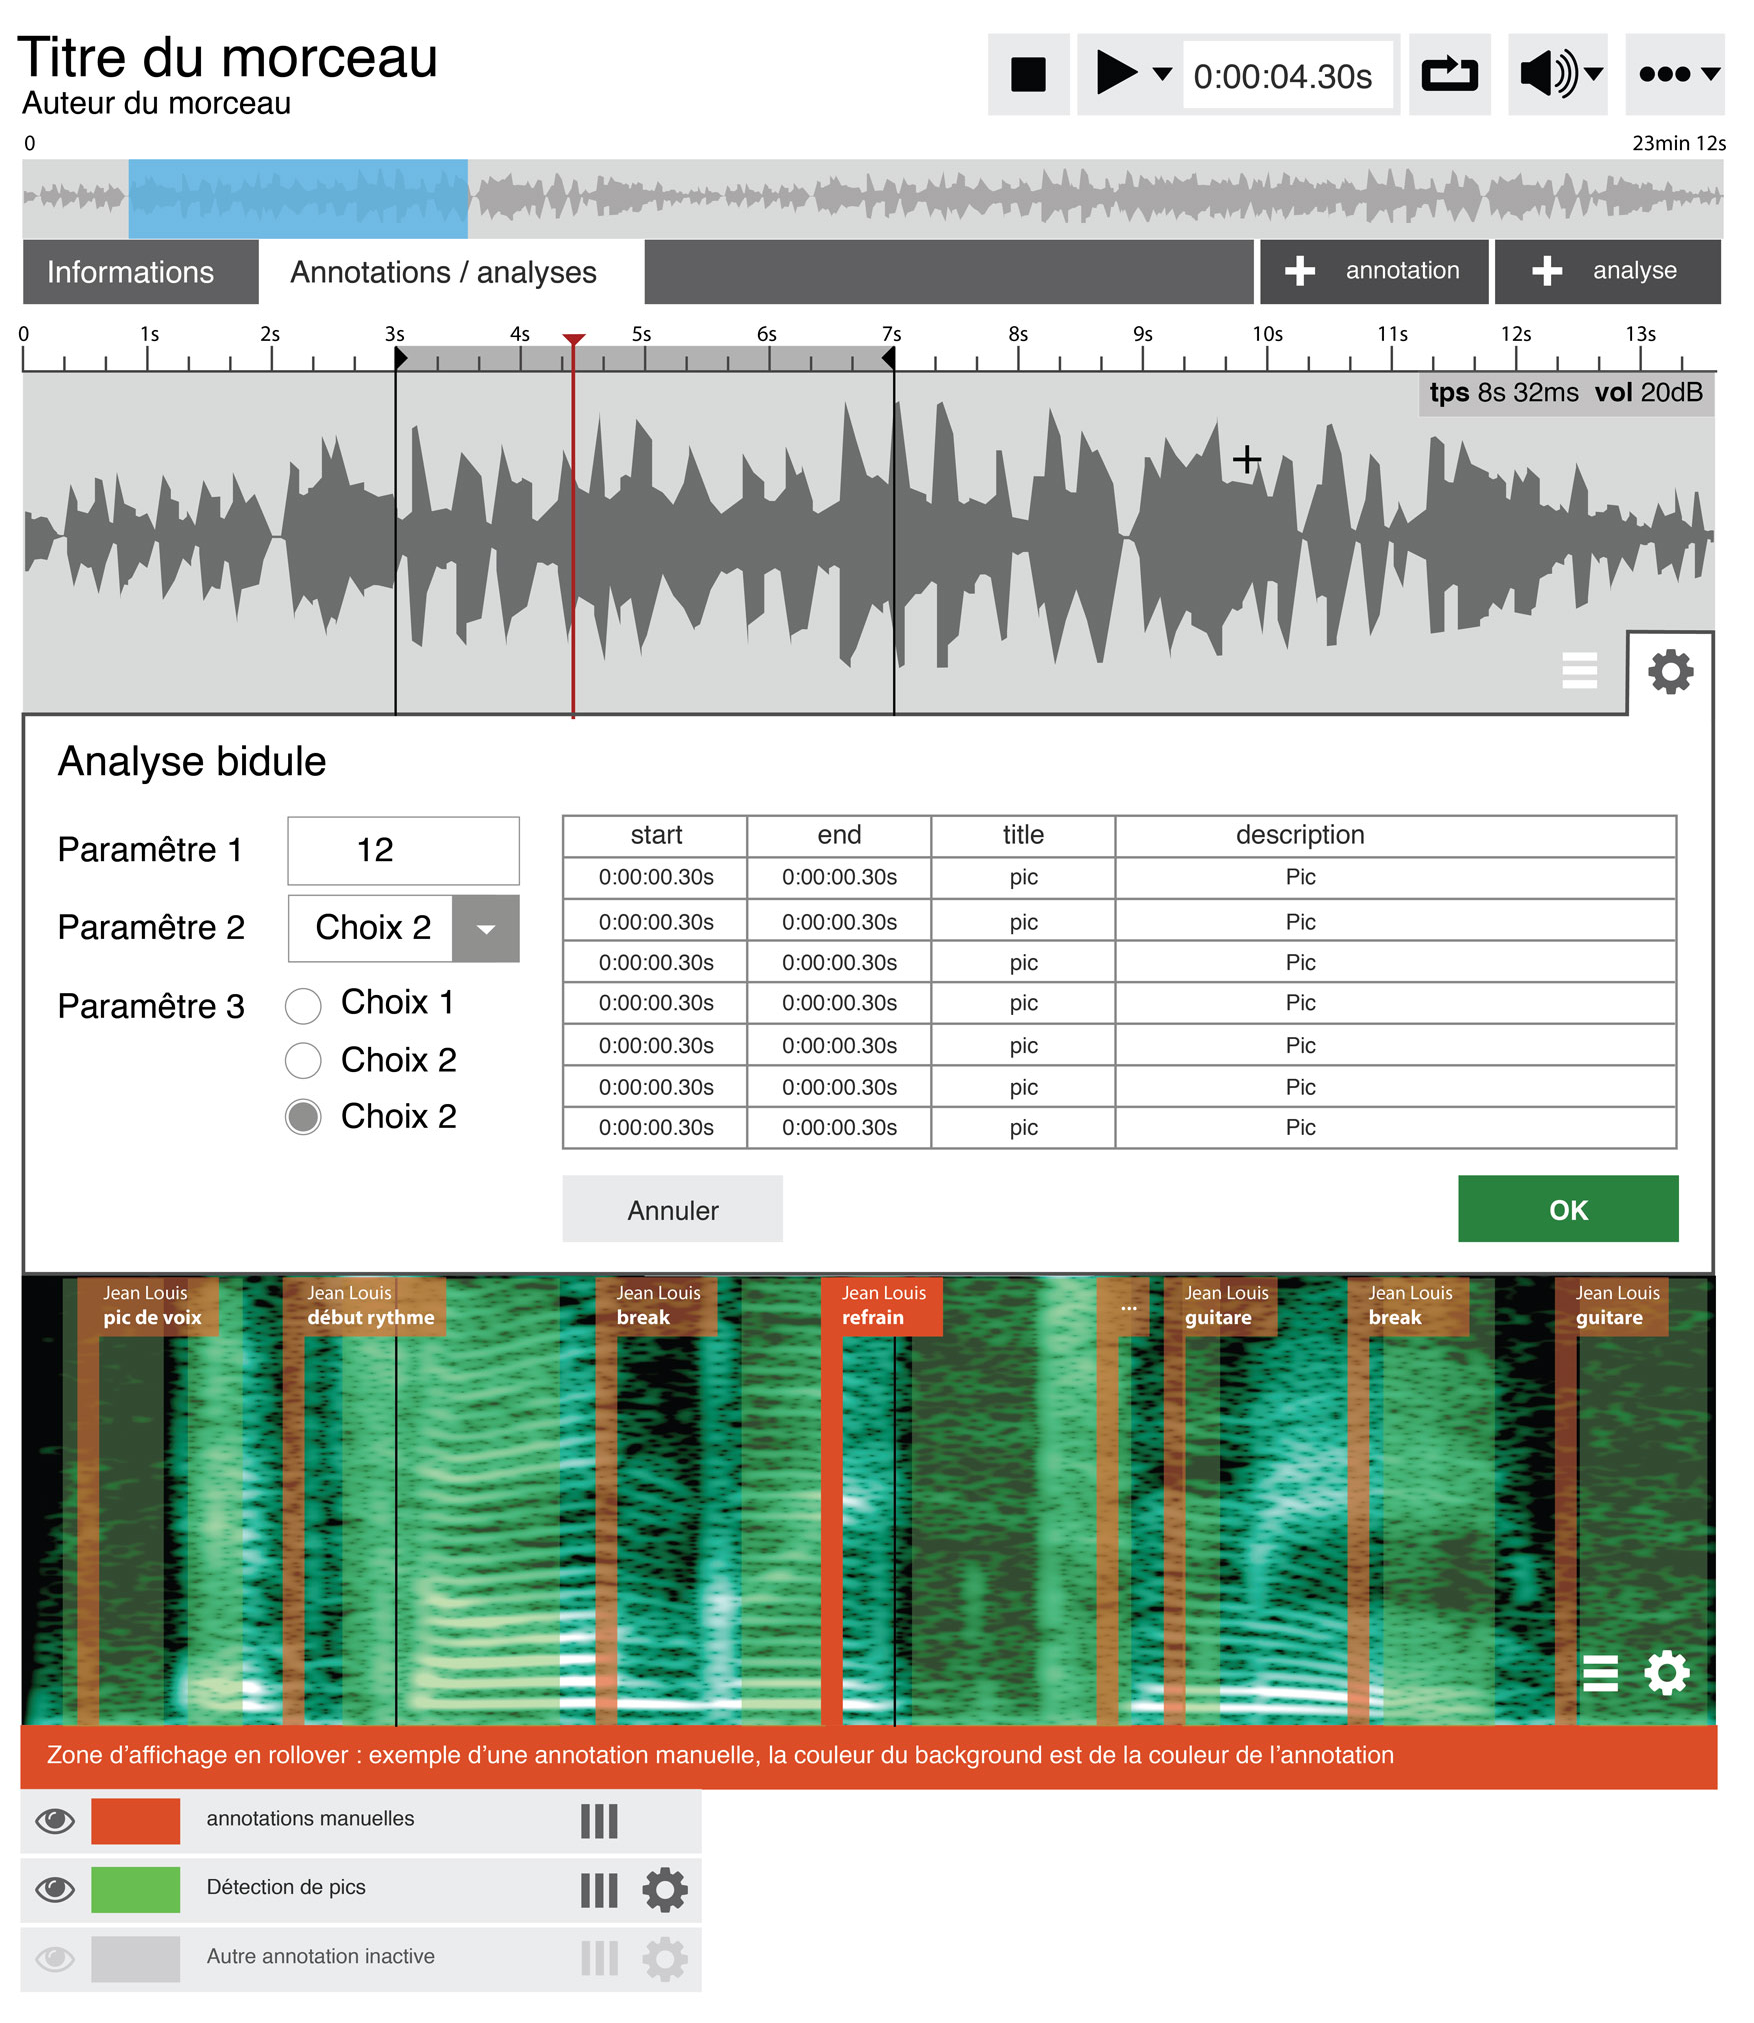
\includegraphics[width=0.93\linewidth]{figs/ui-timeside-grand-2_1.png}}}
 \caption{Sketch of the TimeSide player v2}
 \label{fig:ts_player_v2}
\end{figure}

This work has been followed recently by the context of the WASABI project\footnote{\tiny\url{http://www.agence-nationale-recherche.fr/Project-ANR-16-CE23-0017}}: \textit{Web Audio and Semantic Aggregated in the Browser for Indexation} which one aspect is aiming to test the capability on TimeSide to scale on a 2 million music dataset. The resulting consistent data will be linked to a semantical triple store feeded by various strucured data gathered on the Web. It is intended to provided high level interface to various type of users to enhance the musical exploring experience with audio informations as well as structured cultural informations and lyrics.

\section{Conclusion and Future Work}

We proposed a way to modelize an audio web service based on streaming and high level analyses. TimeSide, as an implementation in Python, is now fully usable and deployable. The framework is now in production for various data repositories and is now shared with various partners. It allows not only fast and easy deploying of common libraries and algorithms, but also a flexible way to exchange some structured metadata outcoming from audio analysis when it becomes difficult to share the datasets themselves. We expect that it can reach some new communities, especially in MIR and music industry where the Web is expected to be the central point of providing data. We think that TimeSide is capable of being an original open web service that provides new spaces for the valorisation of AI algorithms - especially \textit{active learning} where expert inputs are needed through innovative and collaborative interfaces - as well as cultural and social data coming from the society.

\section{ACKNOWLEDGMENTS}

The development of TimeSide has received support from the french Center of National Research and Science (CNRS), the Center for Research in Ethnomusilogy (CREM), the DIADEMS, WASABI (ANR-16-CE23-0017) and KAMoulox projects funded by the french National Agency for Research, the DaCaRyH project funded by the Labex ``Les Pass\'es dans le Pr\'esent'' and AHRC with the Queen Mary University of London, the NYU/CREM project funded by the New York University.


\bibliography{ISMIRtemplate}

\end{document}
\grid
\grid
